\documentclass{standalone}
\usepackage{tikz}
\usetikzlibrary{patterns, positioning}
\usepackage[sfdefault]{ClearSans} %% option 'sfdefault' activates Clear Sans as the default text font
\usepackage[T1]{fontenc}

\begin{document}
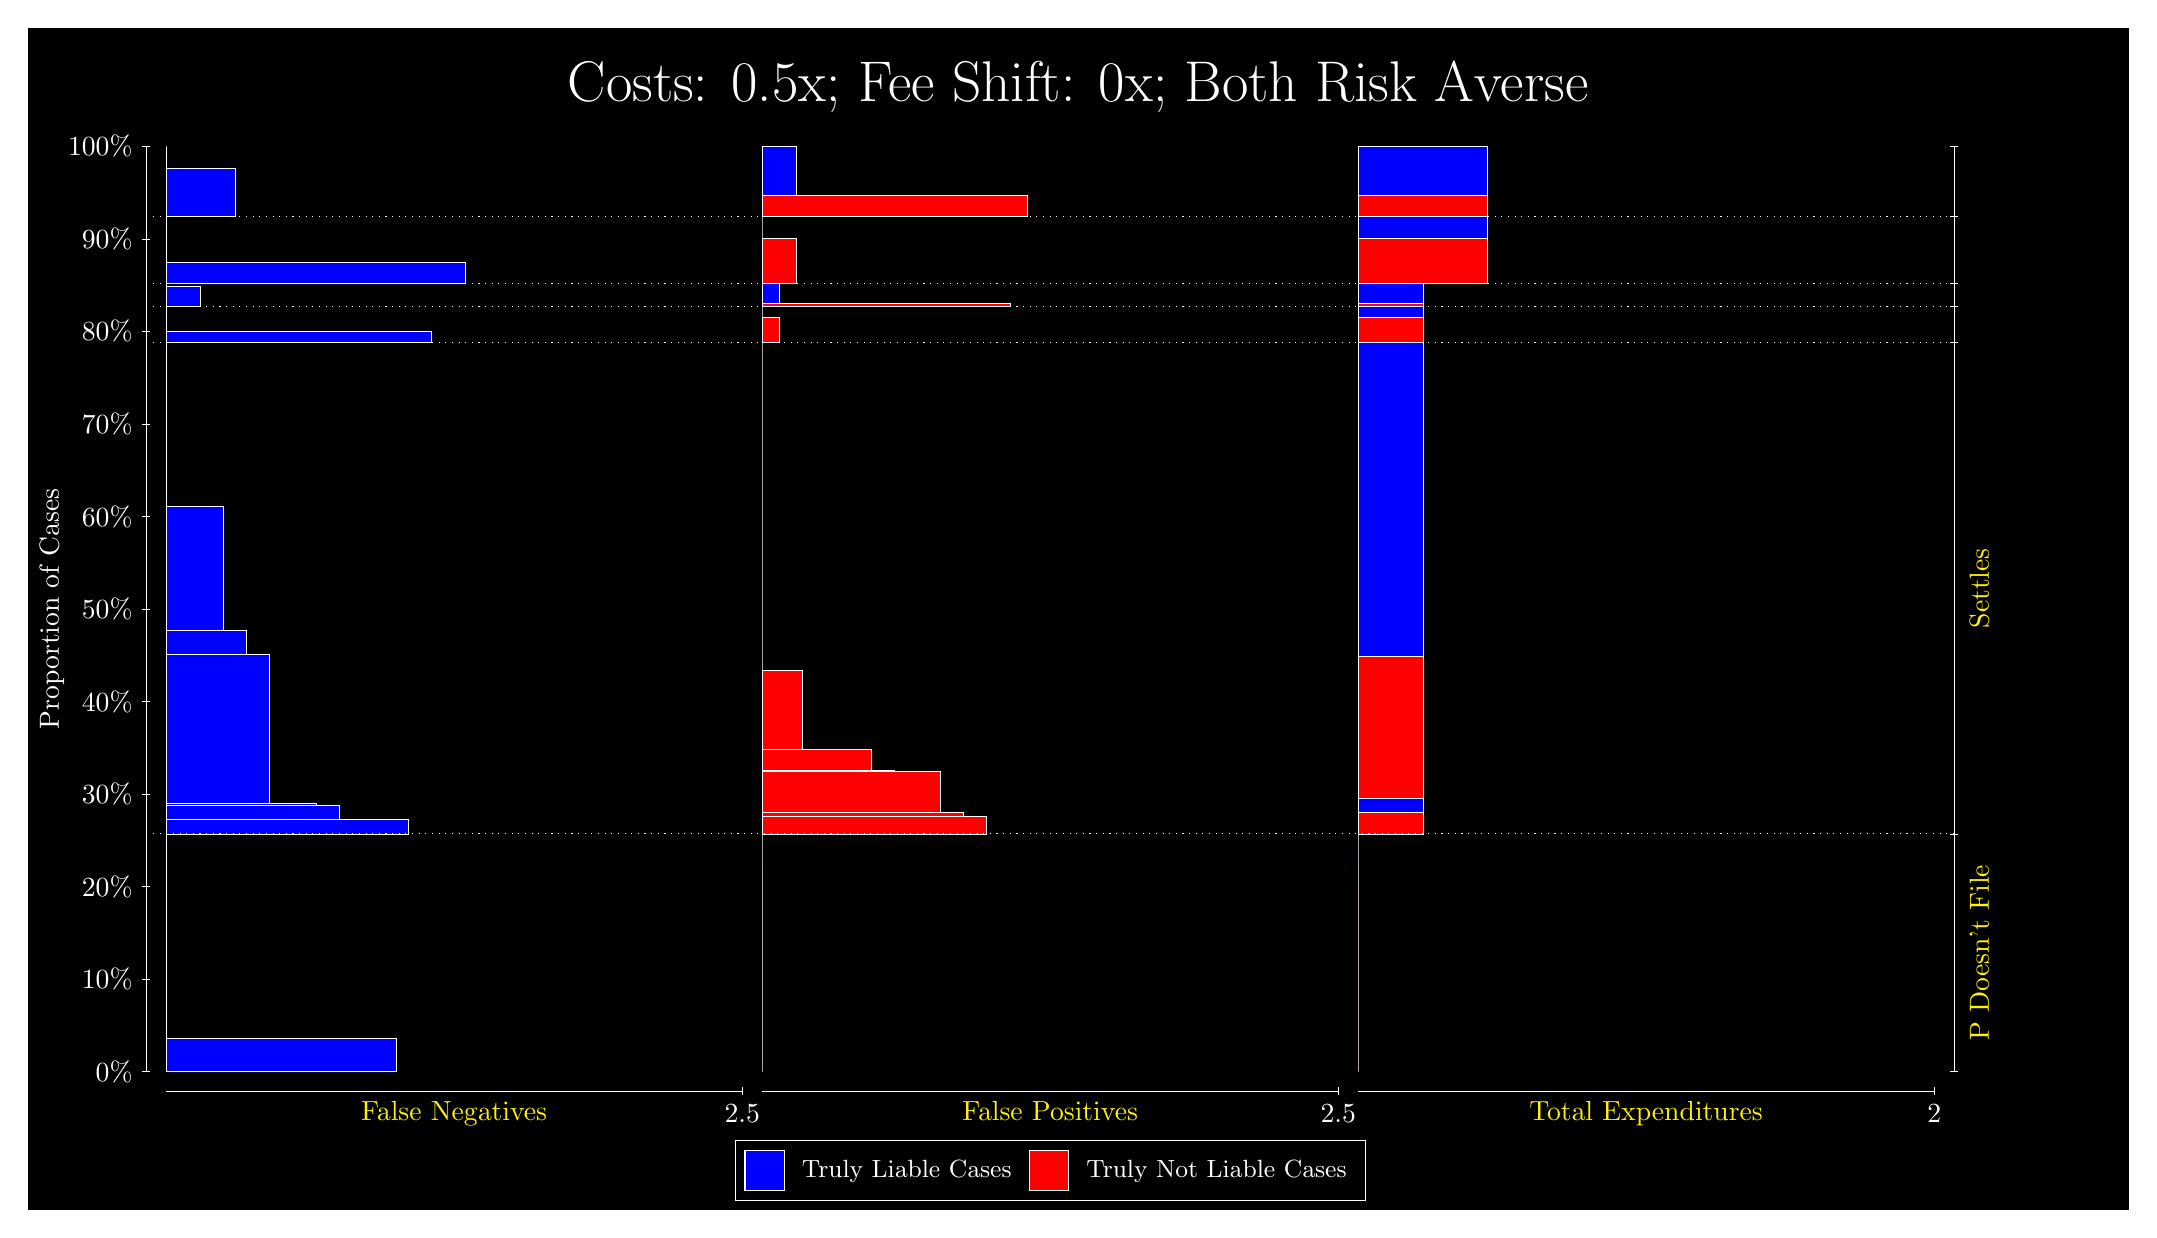
\begin{tikzpicture}
\draw[fill=black] (0,0) rectangle (26.667,15);
\draw[text=white] (0,13.5) rectangle (26.667,15) node[midway] {\huge Costs: 0.5x; Fee Shift: 0x; Both Risk Averse};
\draw[white, very thin] (1.5,1.75) -- (1.5,13.5);
\node[rotate=90, text=white, anchor=center] at (0.3, 7.625) {Proportion of Cases};
\draw[white, very thin] (1.45,1.75) -- (1.55,1.75);
\node[text=white, anchor=east] at (1.45, 1.75) {0\%};
\draw[white, very thin] (1.45,2.925) -- (1.55,2.925);
\node[text=white, anchor=east] at (1.45, 2.925) {10\%};
\draw[white, very thin] (1.45,4.1) -- (1.55,4.1);
\node[text=white, anchor=east] at (1.45, 4.1) {20\%};
\draw[white, very thin] (1.45,5.275) -- (1.55,5.275);
\node[text=white, anchor=east] at (1.45, 5.275) {30\%};
\draw[white, very thin] (1.45,6.45) -- (1.55,6.45);
\node[text=white, anchor=east] at (1.45, 6.45) {40\%};
\draw[white, very thin] (1.45,7.625) -- (1.55,7.625);
\node[text=white, anchor=east] at (1.45, 7.625) {50\%};
\draw[white, very thin] (1.45,8.8) -- (1.55,8.8);
\node[text=white, anchor=east] at (1.45, 8.8) {60\%};
\draw[white, very thin] (1.45,9.975) -- (1.55,9.975);
\node[text=white, anchor=east] at (1.45, 9.975) {70\%};
\draw[white, very thin] (1.45,11.15) -- (1.55,11.15);
\node[text=white, anchor=east] at (1.45, 11.15) {80\%};
\draw[white, very thin] (1.45,12.325) -- (1.55,12.325);
\node[text=white, anchor=east] at (1.45, 12.325) {90\%};
\draw[white, very thin] (1.45,13.5) -- (1.55,13.5);
\node[text=white, anchor=east] at (1.45, 13.5) {100\%};

\draw[white, very thin] (24.457,1.75) -- (24.457,13.5);
\draw[white, very thin] (24.407,1.75) -- (24.507,1.75);
\node[anchor=west] at (24.407, 1.75) {};
\draw[white, very thin] (24.407,4.7682) -- (24.507,4.7682);
\node[anchor=west] at (24.407, 4.7682) {};
\draw[white, very thin] (24.407,11.007) -- (24.507,11.007);
\node[anchor=west] at (24.407, 11.007) {};
\draw[white, very thin] (24.407,11.47) -- (24.507,11.47);
\node[anchor=west] at (24.407, 11.47) {};
\draw[white, very thin] (24.407,11.755) -- (24.507,11.755);
\node[anchor=west] at (24.407, 11.755) {};
\draw[white, very thin] (24.407,12.606) -- (24.507,12.606);
\node[anchor=west] at (24.407, 12.606) {};
\draw[white, very thin] (24.407,13.5) -- (24.507,13.5);
\node[anchor=west] at (24.407, 13.5) {};

\draw[white, very thin, fill=blue] (1.75,1.75) rectangle (4.6775,2.172);
\draw[white, very thin, fill=red] (1.75,2.172) rectangle (1.75,4.7682);
\draw[white, very thin, fill=blue] (1.75,4.7682) rectangle (4.8239,4.9473);
\draw[white, very thin, fill=blue] (1.75,4.9473) rectangle (3.9457,5.1293);
\draw[white, very thin, fill=blue] (1.75,5.1293) rectangle (3.6529,5.1521);
\draw[white, very thin, fill=blue] (1.75,5.1521) rectangle (3.0674,7.0431);
\draw[white, very thin, fill=blue] (1.75,7.0431) rectangle (2.7746,7.3525);
\draw[white, very thin, fill=blue] (1.75,7.3525) rectangle (2.4819,8.9336);
\draw[white, very thin, fill=red] (1.75,8.9336) rectangle (1.75,11.007);
\draw[white, very thin, fill=blue] (1.75,11.007) rectangle (5.1167,11.147);
\draw[white, very thin, fill=red] (1.75,11.147) rectangle (1.75,11.47);
\draw[white, very thin, fill=blue] (1.75,11.47) rectangle (2.1891,11.724);
\draw[white, very thin, fill=red] (1.75,11.724) rectangle (1.75,11.755);
\draw[white, very thin, fill=blue] (1.75,11.755) rectangle (5.5558,12.029);
\draw[white, very thin, fill=red] (1.75,12.029) rectangle (1.75,12.606);
\draw[white, very thin, fill=blue] (1.75,12.606) rectangle (2.6283,13.226);
\draw[white, very thin, fill=red] (1.75,13.226) rectangle (1.75,13.5);
\draw[white, very thin, fill=red] (9.3189,1.75) rectangle (9.3189,4.3462);
\draw[white, very thin, fill=blue] (9.3189,4.3462) rectangle (9.3189,4.7682);
\draw[white, very thin, fill=red] (9.3189,4.7682) rectangle (12.173,4.9906);
\draw[white, very thin, fill=red] (9.3189,4.9906) rectangle (11.88,5.0378);
\draw[white, very thin, fill=red] (9.3189,5.0378) rectangle (11.588,5.5617);
\draw[white, very thin, fill=red] (9.3189,5.5617) rectangle (11.002,5.5737);
\draw[white, very thin, fill=red] (9.3189,5.5737) rectangle (10.709,5.8426);
\draw[white, very thin, fill=red] (9.3189,5.8426) rectangle (9.8312,6.8416);
\draw[white, very thin, fill=blue] (9.3189,6.8416) rectangle (9.3189,11.007);
\draw[white, very thin, fill=red] (9.3189,11.007) rectangle (9.5384,11.331);
\draw[white, very thin, fill=blue] (9.3189,11.331) rectangle (9.3189,11.47);
\draw[white, very thin, fill=red] (9.3189,11.47) rectangle (12.466,11.501);
\draw[white, very thin, fill=blue] (9.3189,11.501) rectangle (9.5384,11.755);
\draw[white, very thin, fill=red] (9.3189,11.755) rectangle (9.758,12.332);
\draw[white, very thin, fill=blue] (9.3189,12.332) rectangle (9.3189,12.606);
\draw[white, very thin, fill=red] (9.3189,12.606) rectangle (12.686,12.88);
\draw[white, very thin, fill=blue] (9.3189,12.88) rectangle (9.758,13.5);
\draw[white, very thin, fill=red] (16.888,1.75) rectangle (16.888,4.3462);
\draw[white, very thin, fill=blue] (16.888,4.3462) rectangle (16.888,4.7682);
\draw[white, very thin, fill=red] (16.888,4.7682) rectangle (17.711,5.0371);
\draw[white, very thin, fill=blue] (16.888,5.0371) rectangle (17.711,5.219);
\draw[white, very thin, fill=red] (16.888,5.219) rectangle (17.711,7.0235);
\draw[white, very thin, fill=blue] (16.888,7.0235) rectangle (17.711,11.007);
\draw[white, very thin, fill=red] (16.888,11.007) rectangle (17.711,11.331);
\draw[white, very thin, fill=blue] (16.888,11.331) rectangle (17.711,11.47);
\draw[white, very thin, fill=red] (16.888,11.47) rectangle (17.711,11.501);
\draw[white, very thin, fill=blue] (16.888,11.501) rectangle (17.711,11.755);
\draw[white, very thin, fill=red] (16.888,11.755) rectangle (18.534,12.332);
\draw[white, very thin, fill=blue] (16.888,12.332) rectangle (18.534,12.606);
\draw[white, very thin, fill=red] (16.888,12.606) rectangle (18.534,12.88);
\draw[white, very thin, fill=blue] (16.888,12.88) rectangle (18.534,13.5);
\draw[white, dotted] (1.5,4.7682) -- (24.457,4.7682);
\draw[white, dotted] (1.5,11.007) -- (24.457,11.007);
\draw[white, dotted] (1.5,11.47) -- (24.457,11.47);
\draw[white, dotted] (1.5,11.755) -- (24.457,11.755);
\draw[white, dotted] (1.5,12.606) -- (24.457,12.606);
\draw[white, very thin] (1.75,1.5) -- (9.0689,1.5);
\node[text=yellow, anchor=north] at (5.4094, 1.5) {False Negatives};
\draw[white, very thin] (9.0689,1.45) -- (9.0689,1.55);
\node[text=white, anchor=north] at (9.0689, 1.45) {2.5};

\draw[white, very thin] (9.3189,1.5) -- (16.638,1.5);
\node[text=yellow, anchor=north] at (12.978, 1.5) {False Positives};
\draw[white, very thin] (16.638,1.45) -- (16.638,1.55);
\node[text=white, anchor=north] at (16.638, 1.45) {2.5};

\draw[white, very thin] (16.888,1.5) -- (24.207,1.5);
\node[text=yellow, anchor=north] at (20.547, 1.5) {Total Expenditures};
\draw[white, very thin] (24.207,1.45) -- (24.207,1.55);
\node[text=white, anchor=north] at (24.207, 1.45) {2};

\node[text=yellow, centered, rotate=90] at (24.777, 3.2591) {P Doesn't File};
\node[text=yellow, centered, rotate=90] at (24.777, 7.8876) {Settles};





\draw (12.978300999999998,1.5) node[draw=none] (baseCoordinate) {};
\begin{scope}[align=center]
        \matrix[scale=0.5, draw=white, below=0.5cm of baseCoordinate, nodes={draw}, column sep=0.1cm]{
            \node[rectangle, draw, minimum width=0.5cm, minimum height=0.5cm, fill=blue] {}; &
            \node[draw=none, font=\small, text=white] (B) {Truly Liable Cases}; &
            \node[rectangle, draw, minimum width=0.5cm, minimum height=0.5cm, fill=red] {}; &
            \node[draw=none, font=\small, text=white] (B) {Truly Not Liable Cases}; \\
            };
\end{scope}

\end{tikzpicture}
\end{document}